\subsection{Descripción del problema.}

\vspace*{0.3cm}

Se tiene un juego de mesa cuyo tablero, dividido en casillas, posee igual cantidad de filas y columnas y hace uso de una conocida pieza del popular ajedrez: el caballo. El juego es solamente para un jugador y consiste en, teniendo caballos ubicados en distintos casilleros, insertar en casilleros vacíos la mínima cantidad de caballos extras, de manera tal que, siguendo las reglas del movimiento de los caballos en el ajedrez, todas las casillas se encuentren ocupadas o amenazadas por un caballo.
Aspectos a tener en cuenta:

\begin{itemize}
   \item Se conoce la cantidad de filas y columnas del tablero
   \item Se conoce la cantidad de caballos que ocupan el tablero inicialmente.
   \item Para cada uno de estos caballos, se sabe su ubicación en el tablero
   \item Una casilla se considera amenazada si existe un caballo tal que en una movida pueda ocupar dicha casilla
\end{itemize}

%\begin{figure}[htb]
%  \begin{center}
%      \includegraphics[scale=0.25]{imagenes/ejemplo.jpg}
%  \end{center}
%  \caption{ejemplo}
%\end{figure}

\vspace*{0.6cm}

%\newpage
\subsection{Desarrollo de la idea y pseudocódigo.}


\begin{figure}[!htb]
\minipage{0.32\textwidth}
  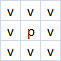
\includegraphics[scale=1]{imagenes/tab1.png}
  \caption{Tablero 1}\label{fig:tab1}
\endminipage\hfill
\minipage{0.32\textwidth}
  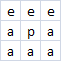
\includegraphics[scale=1]{imagenes/tab2.png}
  \caption{Tablero 2}\label{fig:tab2}
\endminipage\hfill
\minipage{0.32\textwidth}%
  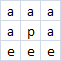
\includegraphics[scale=1]{imagenes/tab3.png}
  \caption{Tablero 3}\label{fig:tab3}
\endminipage
\end{figure}

%\begin{figure}[htb]
 % \begin{center}
%     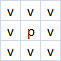
\includegraphics[scale=1]{imagenes/tab1.png}
%  \end{center}
 % \caption{Tablero 1}\label{fig:tab1}
%\end{figure}
%\vspace*{0.3cm}

%\begin{figure}[htb]
 % \begin{center}
  %    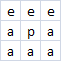
\includegraphics[scale=1]{imagenes/tab2.png}
  %\end{center}
  %\caption{Tablero 2}\label{fig:tab2}
%\end{figure}

%\begin{figure}[htb]
 % \begin{center}
  %    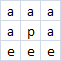
\includegraphics[scale=1]{imagenes/tab3.png}
  %\end{center}
  %\caption{Tablero 3}\label{fig:tab3}
%\end{figure}

Supongamos un ejemplo como el del Figura \ref{fig:tab1}, donde 'v' indica casillero vacío y 'p' un caballo preubicado. Observemos que tanto Figura \ref{fig:tab2} y Figura \ref{fig:tab3} son soluciones (donde 'e' indica que se agrego un caballo extra y 'a' que dicha casilla esta amenazada sin un caballo colocado). Esto significa que en principio, puede haber múltiples soluciones óptimas. Más aún, veamos que si el tablero fuera de $2*2$, la única manera de obtener un tablero completo (diremos que un tablero está completo si todas sus casillas, o tienen un caballo, o están amenazadas por uno) es que haya un caballo en cada casilla, osea que puedo tener soluciones óptimas como en $3x3$ o puedo necesitar completar el tablero con caballos como en $2x2$. Y si fuera de $4*4$?.


\begin{figure}[!htb]
\minipage{0.32\textwidth}
  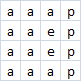
\includegraphics[scale=1]{imagenes/tab4.png}
  \caption{Tablero 4}\label{fig:tab4}
\endminipage\hfill
\minipage{0.32\textwidth}
  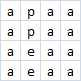
\includegraphics[scale=1]{imagenes/tab5.png}
  \caption{Tablero 5}\label{fig:tab5}
\endminipage\hfill
\minipage{0.32\textwidth}%
  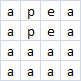
\includegraphics[scale=1]{imagenes/tab6.png}
  \caption{Tablero 6}\label{fig:tab6}
\endminipage
\end{figure}

%\begin{figure}[htb]
% \begin{center}
%    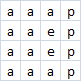
\includegraphics[scale=1]{imagenes/tab4.png}
%  \end{center}
%  \caption{Tablero 4}\label{fig:tab4}
%\end{figure}

%\begin{figure}[htb]
%  \begin{center}
%      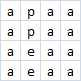
\includegraphics[scale=1]{imagenes/tab5.png}
%  \end{center}
%  \caption{Tablero 5}\label{fig:tab5}
%\end{figure}

%\begin{figure}[htb]
%  \begin{center}
%      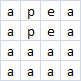
\includegraphics[scale=1]{imagenes/tab6.png}
%  \end{center}
%  \caption{Tablero 6}\label{fig:tab6}
%\end{figure}

\begin{figure}[!htb]
\minipage{0.32\textwidth}
  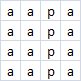
\includegraphics[scale=1]{imagenes/tab7.png}
  \caption{Tablero 7}\label{fig:tab7}
\endminipage
\minipage{0.32\textwidth}
  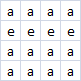
\includegraphics[scale=1]{imagenes/tab8.png}
  \caption{Tablero 8}\label{fig:tab8}
\endminipage
\end{figure}

%\begin{figure}[htb]
%  \begin{center}
%      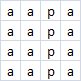
\includegraphics[scale=1]{imagenes/tab7.png}
%  \end{center}
%  \caption{Tablero 7}\label{fig:tab7}
%\end{figure}

%\begin{figure}[htb]
%  \begin{center}
%      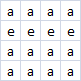
\includegraphics[scale=1]{imagenes/tab8.png}
%  \end{center}
%  \caption{Tablero 8}\label{fig:tab8}
%\end{figure}

Notamos que Figura \ref{fig:tab4} es un ejemplo en el que pude insertar 2 caballos, que tanto Figura \ref{fig:tab5} como Figura \ref{fig:tab6} son solución de un mismo caso inicial (el tablero que tiene solo los caballos preubicados), y que en el Figura \ref{fig:tab7} no es necesario agregar ningún caballo extra. Esto significa que hay casos muy variados y amplios, lo cual vuelve difícil construir un algorítmo que resuelva el problema. Ante esto, como somos malos perdedores, decidimos sacrificar tiempo, pero vamos a encontrar una solución óptima.\\
Podemos afrontar este problema aplicando la técnica de backtracking, planteando un algoritmo que chequee todas las posibles formas de insertar caballos en un determinado tablero, desde rellenar un tablero con caballos hasta no poner ninguno, y se quede con una solución tal que el tablero esté completo y la cantidad de caballos insertados sea menor o igual al de todo el resto de las soluciones.\\
Una idea más ordenada de este algoritmo de backtracking es la siguiente (suponiendo que el tablero de entrada no está completo, puesto que sino se devolverá este mismo tablero):
\begin{itemize}
\item Recorriendo el tablero: empezamos por el casillero de la primera fila y columna para ir avanzando por los distintos casilleros de esa fila, en orden, y cuando se llegue al final de una fila, continuaremos por el primer casillero de la fila siguiente. De esta manera, recorremos el tablero completo, asegurandome que se pasa por todas las casillas (A).
\item Insertando caballos: para cada casillero, si este tiene un caballo "p" colocado, se verá el siguiente casillero, y de no existir, la solución dada hasta el momento se tomará como la óptima. Sino, abordaremos dos posibilidades. Primero veremos el caso en el que se coloca un caballo en ese casillero, y después veremos el caso en el que no se agrega dicho caballo \ref{fig:diag}. En cada caso, se verá si el tablero queda o no completo, y si queda completo, se lo comparará con el resto de las soluciones completas, para ver si la cantidad de caballos agregados es menor o igual a todas o no. En caso de serlo, se la considerará la solución hasta que se encuentre otra mejor. De no encontrarse una solución mejor en los siguientes casos que se observen, será considerada mi solución óptima. Junto con (A), esto significa que se ven todas las posibles ramas de decisión \ref{fig:diag}, y por cada decisión se pregunta si es una solución, y si lo es, si es mejor que las anteriores, lo que quiere decir que pregunta por todas las soluciones y se queda con la mejor efectivamente.
\end{itemize}
\begin{figure}[htb]
  \begin{center}
      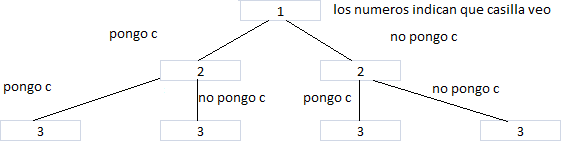
\includegraphics[scale=1]{imagenes/tab9.png}
  \end{center}
  \caption{Diagrama de acción}\label{fig:diag}
\end{figure}

Teniendo en cuenta estos métodos, llegamos a la conclusión de que nuestro algoritmo es correcto, sin embargo, ver todos los casos resulta tedioso y si bien tenemos tiempo, los docentes de algo 3 se molestarían si perdemos demasiado, lo cual motiva a aplicar cotas estratégicas. Estas funcionarán de la siguiente manera, si un caso dado supera a la cota, se desechará, puesto que ese camino seguro no llega a una solución óptima. De encontrarse una solución que mejora a la cota, entonces esta solución pasará a ser la nueva cota.\\
Analizemos que cotas tomar:\\
No podemos pensar un caso por cada tamaño de tablero, puesto que no terminaría nunca, pero si podemos pensar que si vemos el Tablero \ref{fig:tab1} y reemplazamos la 'p' por una 'v', la solución Tablero \ref{fig:tab2} es óptima (cambiando su 'p' por una 'e' ) lo cual significa que independientemente de los caballos 'p', con a lo sumo 4 se debe completar un tablero. Por otro lado, como mencionamos previamente, a un tablero de $2*2$ hay que llenarlo de caballos, y si vemos el Tablero \ref{fig:tab8}, vemos que a un tablero de $4*4$ vacío, con 4 caballos le basta para completarse, lo cual indica que sucede algo similar con el tablero de $3*3$. Por esto diremos que si nuestro tablero es menor o igual a $4*4$, no debo ver aquellos casos que pongan más de 4 caballos, puesto que de seguro, eso no es una solución óptima.¿ Pero qué sucede con el resto de los casos?. Observemos lo siguiente, sea un tablero de $n*m$ (no apto para este juego, pero si para lo que se quiere mostrar) con  $n=5$ y $m\geq5$. Tomemos por ejemplo un tablero de $5*5$ vacío, pero con una fila de caballos en el centro (llamados c).


\begin{figure}[!htb]
\minipage{0.32\textwidth}
  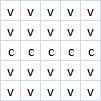
\includegraphics[scale=1]{imagenes/tab10.png}
  \caption{Tablero 10}\label{fig:tab10}
\endminipage
\minipage{0.32\textwidth}
  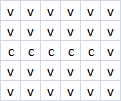
\includegraphics[scale=1]{imagenes/tab11.png}
  \caption{Tablero 11}\label{fig:tab11}
\endminipage
\end{figure}

%\begin{figure}[htb]
%  \begin{center}
%      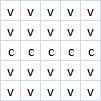
\includegraphics[scale=1]{imagenes/tab10.png}
%  \end{center}
%  \caption{Tablero 9}\label{fig:tab9}
%\end{figure}

%\begin{figure}[htb]
%  \begin{center}
%      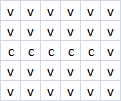
\includegraphics[scale=1]{imagenes/tab11.png}
%  \end{center}
%  \caption{Tablero 10}\label{fig:tab10}
%\end{figure}

Notemos que en Figura \ref{fig:tab9} todas las casillas están amenazadas u ocupadas y sería un tablero completo. Es más, si sacaramos un solo caballo, el tablero dejaría de ser completo. Esto, si bien no tiene por que ser un óptimo, es cuando menos una solución que no usa una cantidad abusiva de caballos.¿ Qué sucederia si extendieramos una columna más, como en Figura \ref{fig:tab10}?. Todas las casillas estarían ocupadas menos la de la fila del medio a la derecha. Osea que si la fila estuviera completa, sería un tablero completo. Nótese que si vuelvo a extender una columna sucede lo mismo. Volviendo otra vez a tableros válidos, la idea recien mencionada nos hace pensar que independientemente del tamaño del tablero, con una línea de caballos cada 5 filas, debería bastar para completar el tablero, y ver más caballos que eso sería un esfuerzo innecesario. Esto se debe a que si el tablero no fuera múltiplo de 5, basta con poner 1 fila de caballos cada 5 filas normales, y de lo que me queda elijo una fila que sea céntrica respecto de las sobrantes, que son menores que 5, y la convierto en fila de caballos. Ver que si una fila céntrica completa 5 filas, en particular completa 4,3,2 y 1.
Por todo lo dicho anteriormente, si llamamos n a la cantidad de filas y columnas de un tablero, dado un tablero de $n*n$ con $n<5$, tomo como cota 4 caballos extras, y si $n\geq5$ tomo como cota n* redondeado_hacia_arriba($\frac{n}{5}$) que resultaría de meter una fila de caballos por cada 5 filas del tablero.\\
¿Sin embargo, agregar estas cotas, puede producir que obtenga un resultado no óptimo?. La pregunta casi que se contesta sola, pues las cotas justamente se basan en que conozco una solución segura que no se si es óptima, pero se que usa una determinada cantidad de caballos, y una solución que use más caballos que esta seguro no es óptima.
%\textbf{completar!}

%\begin{codebox}
%\Procname{$\proc{ejemplo_de_pseudocodigo}(x,y)$}
%\li \Return $\id{solucion}$
%\end{codebox}

\vspace*{0.6cm}

%\newpage
\subsection{Justificación de la resolución y demostración de correctitud.}

\vspace*{0.3cm}

%\textbf{completar!}

\vspace*{0.6cm}

%\newpage
\subsection{Análisis de complejidad.}

\vspace*{0.3cm}


\begin{figure}
\begin{codebox}
\Procname{$\proc{Backtracking}(Tablero$ $tab, Tablero$ $tab$_$final, int$ $fila, int$ $columna, int$ $n)$}
\li copia_tab $\leftarrow$ tablero vacío de n x n // $\mathcal{O}(1)$
\li \If agregué más caballos de los que permitía la cota   // $\mathcal{O}(1)$
\li \quad \Return   
\li \If ya llené el tablero                                // $\mathcal{O}(1)$
\li \quad tab_final $\leftarrow$ copia de tab              // $\mathcal{O}(n^2)$
\li \quad cota $\leftarrow$ cantidad de caballos agregados        // $\mathcal{O}(1)$
\li \quad \Return
\li \If ya recorrí todo el tablero
\li \quad \Return
\li f $\leftarrow$ fila para la siguiente llamada recursiva  // $\mathcal{O}(1)$
\li c $\leftarrow$ columna para la siguiente llamada recursiva  // $\mathcal{O}(1)$
\li \If en tab[fila][columna] no había un caballo preubicado      // $\mathcal{O}(1)$
\li \quad copia_tab $\leftarrow$ copia de tab              // $\mathcal{O}(n^2)$
\li \quad r $\leftarrow$ cantidad de casillas que falta llenar  //$\mathcal{O}(1)$
\li \quad e $\leftarrow$ cantidad de caballos agregados hasta ahora $\mathcal{O}(1)$
\li \quad \If copia_tab[fila][columna] no está cubierta
\li \quad \quad r- -
\li \quad copia_tab[fila][columna] $\leftarrow$ coloco un caballo extra y setea las casillas que amenaza ese nuevo caballo extra    \\   // $\mathcal{O}(1)$
\li \quad e++          // $\mathcal{O}(1)$
\li \quad {\it Backtraking}(copia_tab,tab_final,f,c,n) \\
//Hago la llamada recursiva a backtracking con el nuevo tablero y los datos actualizados \\
teniendo en cuenta el caballo extra
\li {\it Backtraking}(tab,tab_final,f,c,n)\\
//Llamo a backtracking con el tablero nuevo que no tiene asignado el caballo extra
\end{codebox}
\caption{Pseudocódigo del backtraking}\label{code:backtraking}
\end{figure}
\FloatBarrier

\begin{figure}
\begin{codebox}
\Procname{$\proc{El_señor_de_los_caballos}$} 
\li n $\leftarrow$ tamaño del tablero //tomado por la entrada estándar
\li k $\leftarrow$ cantidad de caballos preubicados //tomado por la entrada estándar
\li extras $\leftarrow$ 0
\li tab $\leftarrow$ tablero de n x n vacío // $\mathcal{O}(1)$
\li tab_final $\leftarrow$ tablero de n x n vacío donde irá el resultado // $\mathcal{O}(1)$
\li tab $\leftarrow$ setear ubicación de los caballos preubicadosy las casillas que amenaza cada uno.
\li falta_cubrir $\leftarrow$ cantidad de casillas no ocupadas $\mathcal{O}(1)$
\li \If ($n < 5$)
\li \quad cota $\leftarrow$ 4  // $\mathcal{O}(1)$
\li \Else
\li \quad cota $\leftarrow$ $n*\left \lceil \dfrac{n}{5} \right \rceil$   // $\mathcal{O}(1)$
\li {\it Backtracking}(tab,tab_final,0,0,n)
\li //función que, usando la técnica de backtracking arma el tablero de salida y calcula en\\ extras la cantidad de caballos agregados
\li Muestro por pantalla: cantidad de caballos agregados\\la posición de cada caballo extra
\end{codebox}
\caption{Pseudocódigo de El señor de los caballos}\label{code:caballos}
\end{figure}
\FloatBarrier

Ahora procederemos a demostrar que el algoritmo que planteamos posee una complejidad de $\mathcal{O}(n^2*2^{n^2})$. Luego de un simple vistazo al pseudocodigo (Figura \ref{code:caballos}) se puede ver que la complejidad deriva en gran medida de lo que sucede cuando se llama a la función encargada del backtracking, dado que las comparaciones realizadas son $\mathcal{O}(1)$ asi como las asignaciones. La complejidad de copiar la entrada y generar el tablero adecuado nos resulta $\mathcal{O}(n^2)$.\\
Analicemos ahora un caso particular, como el de un tablero de 2x2 sin caballos preubicados. Haciendo un leve seguimiento del pseudocodigo (Figura \ref{code:backtraking}) nos encontramos revisando la primer casilla del tablero y dado que no hay un caballo preubicado se generan 2 instancias, un nuevo tablero con un caballo extra en esa posicion y otro en el que este no se encuentra presente. La creación de este nuevo tablero nos cuesta $\mathcal{O}(n^2)$. Sobre estas dos instancias se vuelve a llamar a la función de backtracking y el proceso se repite ahora con la casilla siguiente, y asi hasta cubrir las $n*n$ casillas. Al terminar el recorrido notamos que contamos con 15 instancias ($2^{n^2} - 1$) y que por cada una tenemos un costo de $\mathcal{O}(n^2)$.
Este proceso de recorrer todas las casillas se repite para cualquier tablero vacío, creando $2^n -1$ instancias y llegando a una complejidad de $\mathcal{O}(n^2*2^{n^2})$ (el -1 es despreciable).\\
Ahora lo que sucede cuando contamos con caballos preubicados en un tablero cualquiera es que la comparación realizada en la linea 12 de Figura Backtracking, nos ahorra la creacion y copia del nuevo tablero, restando un $\mathcal{O}(n^2)$ a nuestra complejidad. A su vez, la cantidad de ramas con posibles soluciones se ven reducidas considerablemente resultando en $2^{n^2-k}$ instancias.\\
En conclusión nuestro algoritmo, en el peor caso, dado que no hay caballos prefijados, tiene la complejidad de $\mathcal{O}(n^2*2^{n^2})$.

\vspace*{0.6cm}

%\newpage
\subsection{Experimentación y gráficos.}

\vspace*{0.3cm}

\subsubsection{Test 1}

\vspace*{0.3cm}

\textbf{completar!}


\newpage
\subsubsection{Test 2}

\vspace*{0.3cm}

\textbf{completar!}


\newpage
\subsubsection{Test 3}

\vspace*{0.3cm}

\textbf{completar!}
